\documentclass{article}

% PACKAGES
\usepackage[margin=0.75in]{geometry}
\usepackage{amsmath}
\usepackage{amssymb}
\usepackage{graphicx}
\usepackage{subcaption}
\usepackage{float}

% TITLE
\title{Math 273A - Project 3}
\author{Eric Weise - A09642187}

\begin{document}
\maketitle

\section*{Conjugate Gradient}

My code is hosted at GitHub:\\
{\it https://github.com/ericdweise/math-273a/tree/master/MATH\_273A/projects}

\subsection*{To run:}
\begin{verbatim}$ python3 project3.py\end{verbatim}

\begin{figure}[H]
    \caption{Surface plot of the final solution.}
    \centering
        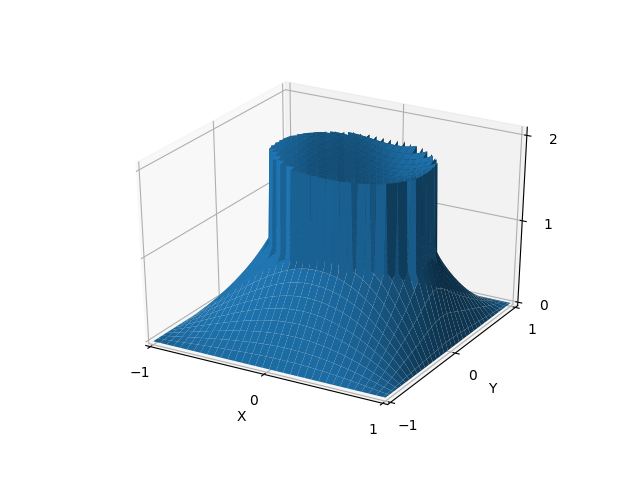
\includegraphics[width=0.5\textwidth]{surface.png}
\end{figure}

\begin{figure}[H]
    \caption{Heatmap of the final surface.}
    \centering
        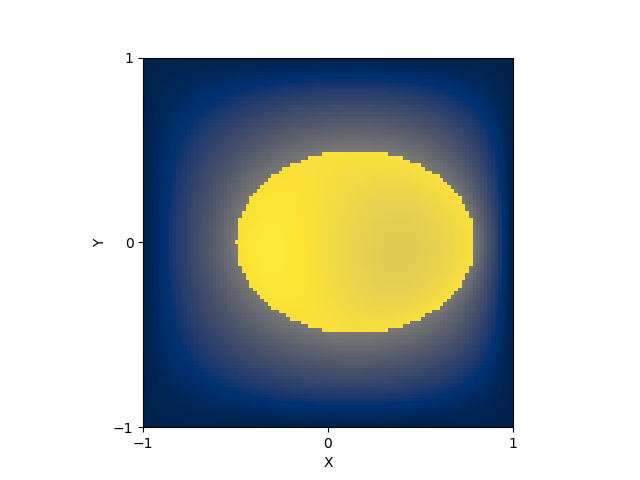
\includegraphics[width=0.5\textwidth]{heatmap.png}
\end{figure}


\end{document}
